%%%%%%%%%%%%%%%%%%%%%%%%%%%%%%%%%%%%%%%%%
% Jacobs Landscape Poster
% LaTeX Template
% Version 1.1 (14/06/14)
%
% Created by:
% Computational Physics and Biophysics Group, Jacobs University
% https://teamwork.jacobs-university.de:8443/confluence/display/CoPandBiG/LaTeX+Poster
%
% Further modified by:
% Nathaniel Johnston (nathaniel@njohnston.ca)
%
% This template has been downloaded from:
% http://www.LaTeXTemplates.com
%
% License:
% CC BY-NC-SA 3.0 (http://creativecommons.org/licenses/by-nc-sa/3.0/)
%
%%%%%%%%%%%%%%%%%%%%%%%%%%%%%%%%%%%%%%%%%

%----------------------------------------------------------------------------------------
%	PACKAGES AND OTHER DOCUMENT CONFIGURATIONS
%----------------------------------------------------------------------------------------

\documentclass[final]{beamer}

\usepackage[scale=1.24]{beamerposter} % Use the beamerposter package for laying out the poster

\usetheme{confposter} % Use the confposter theme supplied with this template

\setbeamercolor{block title}{fg=cmuRed,bg=white} % Colors of the block titles
\setbeamercolor{block body}{fg=black,bg=white} % Colors of the body of blocks
\setbeamercolor{block alerted title}{fg=white,bg=dblue!70} % Colors of the highlighted block titles
\setbeamercolor{block alerted body}{fg=black,bg=dblue!10} % Colors of the body of highlighted blocks
% Many more colors are available for use in beamerthemeconfposter.sty

%-----------------------------------------------------------
% Define the column widths and overall poster size
% To set effective sepwid, onecolwid and twocolwid values, first choose how many columns you want and how much separation you want between columns
% In this template, the separation width chosen is 0.024 of the paper width and a 4-column layout
% onecolwid should therefore be (1-(# of columns+1)*sepwid)/# of columns e.g. (1-(4+1)*0.024)/4 = 0.22
% Set twocolwid to be (2*onecolwid)+sepwid = 0.464
% Set threecolwid to be (3*onecolwid)+2*sepwid = 0.708

\newlength{\sepwid}
\newlength{\onecolwid}
\newlength{\twocolwid}
\newlength{\threecolwid}
\setlength{\paperwidth}{48in} % A0 width: 46.8in
\setlength{\paperheight}{36in} % A0 height: 33.1in
\setlength{\sepwid}{0.024\paperwidth} % Separation width (white space) between columns
\setlength{\onecolwid}{0.22\paperwidth} % Width of one column
\setlength{\twocolwid}{0.464\paperwidth} % Width of two columns
\setlength{\threecolwid}{0.708\paperwidth} % Width of three columns
\setlength{\topmargin}{-0.5in} % Reduce the top margin size
%-----------------------------------------------------------

\usepackage{graphicx}  % Required for including images

\usepackage{booktabs} % Top and bottom rules for tables

%----------------------------------------------------------------------------------------
%	TITLE SECTION
%----------------------------------------------------------------------------------------

\title{Hierarchical Latent Space Models for Social Network Analysis} % Poster title

\author{Alex Loewi\textsuperscript{1,4},
  Francisco Ralston\textsuperscript{2},
  Octavio Mesner\textsuperscript{2,3,4}} % Author(s)

\institute{\textsuperscript{1}Public Policy,
  \textsuperscript{2}Engineering \& Public Policy,
  %Carnegie Mellon University;
  \textsuperscript{3}Statistics \& Data Science,
    \textsuperscript{4}Machine Learning
} % Institution(s)

% ----------------------------------------------------------------------------------------

\begin{document}

\newcommand\curly[1]{\left\{#1\right\}}
\newcommand\brac[1]{\left[#1\right]}
\newcommand\paren[1]{\left(#1\right)}
\newcommand\abs[1]{\left|#1\right|}
\newcommand\norm[1]{\left\|#1\right\|}
\newcommand\ang[1]{\left\langle#1\right\rangle}
\newcommand{\R}{\mathbb{R}}
\renewcommand{\P}{\mathbb{P}}
\newcommand{\N}{\mathbb{N}}
\newcommand{\bone}{\mathbf{1}}
\newcommand{\calL}{\mathcal{L}}
\newcommand{\logitinv}{\textrm{logit}^{-1}}

\addtobeamertemplate{block end}{}{\vspace*{2ex}} % White space under blocks
\addtobeamertemplate{block alerted end}{}{\vspace*{2ex}} % White space under highlighted (alert) blocks

\setlength{\belowcaptionskip}{2ex} % White space under figures
\setlength\belowdisplayshortskip{2ex} % White space under equations

\begin{frame}[t] % The whole poster is enclosed in one beamer frame

\begin{columns}[t] % The whole poster consists of three major columns, the second of which is split into two columns twice - the [t] option aligns each column's content to the top

\begin{column}{\sepwid}\end{column} % Empty spacer column

\begin{column}{\onecolwid} % The first column

%----------------------------------------------------------------------------------------
%	OBJECTIVES
%----------------------------------------------------------------------------------------

%  \begin{alertblock}{Key Points}
%    \begin{itemize}
%    \item Determine the underlying association structure
%    \item
%    \item
%    \item
%    \end{itemize}
%
%\end{alertblock}
%
%----------------------------------------------------------------------------------------
%	INTRODUCTION
%----------------------------------------------------------------------------------------

\begin{block}{Introduction}

  \textbf{Multigraphs:}
  ``Parallel'' network models sharing identical nodes but different
  edges connecting nodes, used to model data where
  actors (nodes) maintain varying types of relationships.\\
  \textbf{Social Network Analysis (SNA)}, where nodes represent
  individual people and edges represent differing relationships, such
  as friendship, professional colleague, or facebook connected, for
  example.\\
  \textbf{Problem:} Social science and network analysis rely
  on intuitive and interpretable models. Visualizing the similarities
  between multiple related graphs is challenging.
  \begin{figure}
    \centering
    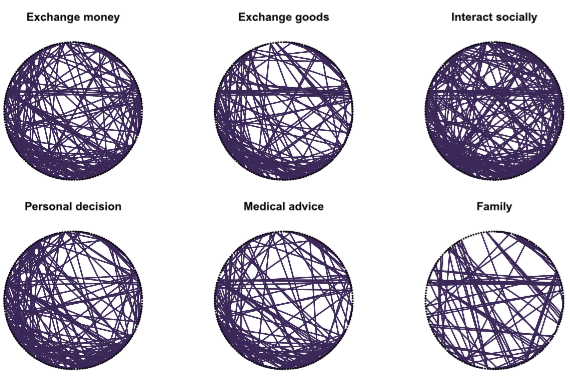
\includegraphics{complexMultigraph.png}
    \caption{(Source: Salter-Townshend, Michael, and Tyler H. McCormick)}
  \end{figure}
  \textbf{Solution:} Using a LASSO penalty, we aim to force similar graphs
  to be displayed in comparable, visualizable, ways
\end{block}

\begin{block}{Employee Relationships Data}
  A recently conducted study at a charter school in West Baltimore\\
  collected a five-layer valued network between the
  approximately eighty employees of the school:
  \begin{itemize}
  \item Frequency of interaction
  \item Discussing Academics
  \item Discussing Behavior
  \item Social interaction
  \item Professionally Helpful Relationship
  \end{itemize}
While empirically these layers are found to have very high
correlations, modeling them in a way that demonstrates those
correlations is challenging.
\end{block}


%------------------------------------------------

%----------------------------------------------------------------------------------------

\end{column} % End of the first column

\begin{column}{\sepwid}\end{column} % Empty spacer column

\begin{column}{\twocolwid} % Begin a column which is two columns wide (column 2)

\begin{columns}[t,totalwidth=\twocolwid] % Split up the two columns wide column

\begin{column}{\onecolwid}\vspace{-.6in} % The first column within column 2 (column 2.1)

%----------------------------------------------------------------------------------------
%	MATERIALS
%----------------------------------------------------------------------------------------

  \begin{block}{Latent Space Projection}
    \begin{itemize}
    \item Map nodes, $i\mapsto z_i\in\R^n$ where proximity,
    $\norm{z_i-z_j}_2=d_{ij}<1$, indicates nodes are connected (and not
    connected otherwise)
    \item Intuitively captures reciprocity ($j\rightarrow i\Rightarrow i\rightarrow j$) and
    transitivity ($i\rightarrow j, j\rightarrow k\Rightarrow
    i\rightarrow k$)
  \item Edge probability: $\sigma_{ij} = \P(Y_{ij}=1|z_i,z_j) = \logitinv\paren{\alpha + \norm{z_i-z_j}_2^2}$
    where $Y_{ij}=1$ indicates $i,j$ are connected in the data, find $z$
  \item Likelihood: $\prod_{i<j} \sigma_{ij}^{y_{ij}}(1- \sigma_{ij})^{1-y_{ij}}$
  \end{itemize}

% The model is based on the widely used Latent Space Model (LSM) for social networks. This model has the following form:

% \[
% \prod_k \prod_{i<j} \sigma_{ijk}^{y_{ijk}}(1- \sigma_{ijk})^{1-y_{ijk}}
% \]

% \[
% \sigma_{ijk} = \text{logit}^{-1}(\alpha_k - d(z_{ik}, z_{jk}))
% \]

% The original model has two simple elements: one, a binomial likelihood for the edges, making for easy and stable inference. And two, an edge probability based on the distance of the two node's latent variables, $z_i, z_j$. The farther apart these variables are, the less likely an edge is. The original model uses the observed edges to infer possible latent positions for the nodes that satisfy these relationships.

\end{block}

%----------------------------------------------------------------------------------------

\end{column} % End of column 2.1

\begin{column}{\onecolwid}\vspace{-.6in} % The second column within column 2 (column 2.2)

%----------------------------------------------------------------------------------------
%	METHODS
%----------------------------------------------------------------------------------------

  \begin{block}{Hierarchical Models}

    \textbf{Goal:} Collapse similar networks indicated by $k$\\
    We include a LASSO penalty on the log-likelihood:
    \begin{align*}
    & \sum_k\sum_{i<j} \brac{y_{ijk} \ln \sigma_{ijk} + (1-y_{ijk})\ln (1-\sigma_{ijk})} \\
    & +\lambda\sum_i \sum_k \norm{\epsilon_{ik}}_1
    \end{align*}
  where $z_{ik} = b_i + \epsilon_{ik}$ for initialization points, $b_i$
% To fit these models, three methods were tested on the following likelihood:

% \[
% \prod_k \prod_{ij} \sigma_{ijk}^{y_{ijk}}(1- \sigma_{ijk})^{1-y_{ijk}} + \lambda\sum_i \sum_k |\epsilon_{ik}|
% \]

\textbf{Optimization Approaches:}
\begin{enumerate}
\item Proximal Gradient Descent
\item Coordinate-Wise Optimization
\item Hamiltonian Monte Carlo methods
\end{enumerate}

%The first was used as a natural approach to the lasso penalized problem, the second was used to prevent the model from ``spinning'' during inference, and the third is the typical way in which these models were fit, used for combarability.

\end{block}

%----------------------------------------------------------------------------------------

\end{column} % End of column 2.2

\end{columns} % End of the split of column 2 - any content after this will now take up 2 columns width

%----------------------------------------------------------------------------------------
%	IMPORTANT RESULT
%----------------------------------------------------------------------------------------

%\begin{alertblock}{Takeaway}
%Convex methods have valuable contributions for fitting complex Latent Space Models, and their extensions
%\end{alertblock}

%----------------------------------------------------------------------------------------
%	RESULTS
%----------------------------------------------------------------------------------------

\begin{block}{Results}

\begin{figure}[h!]
   \centering
   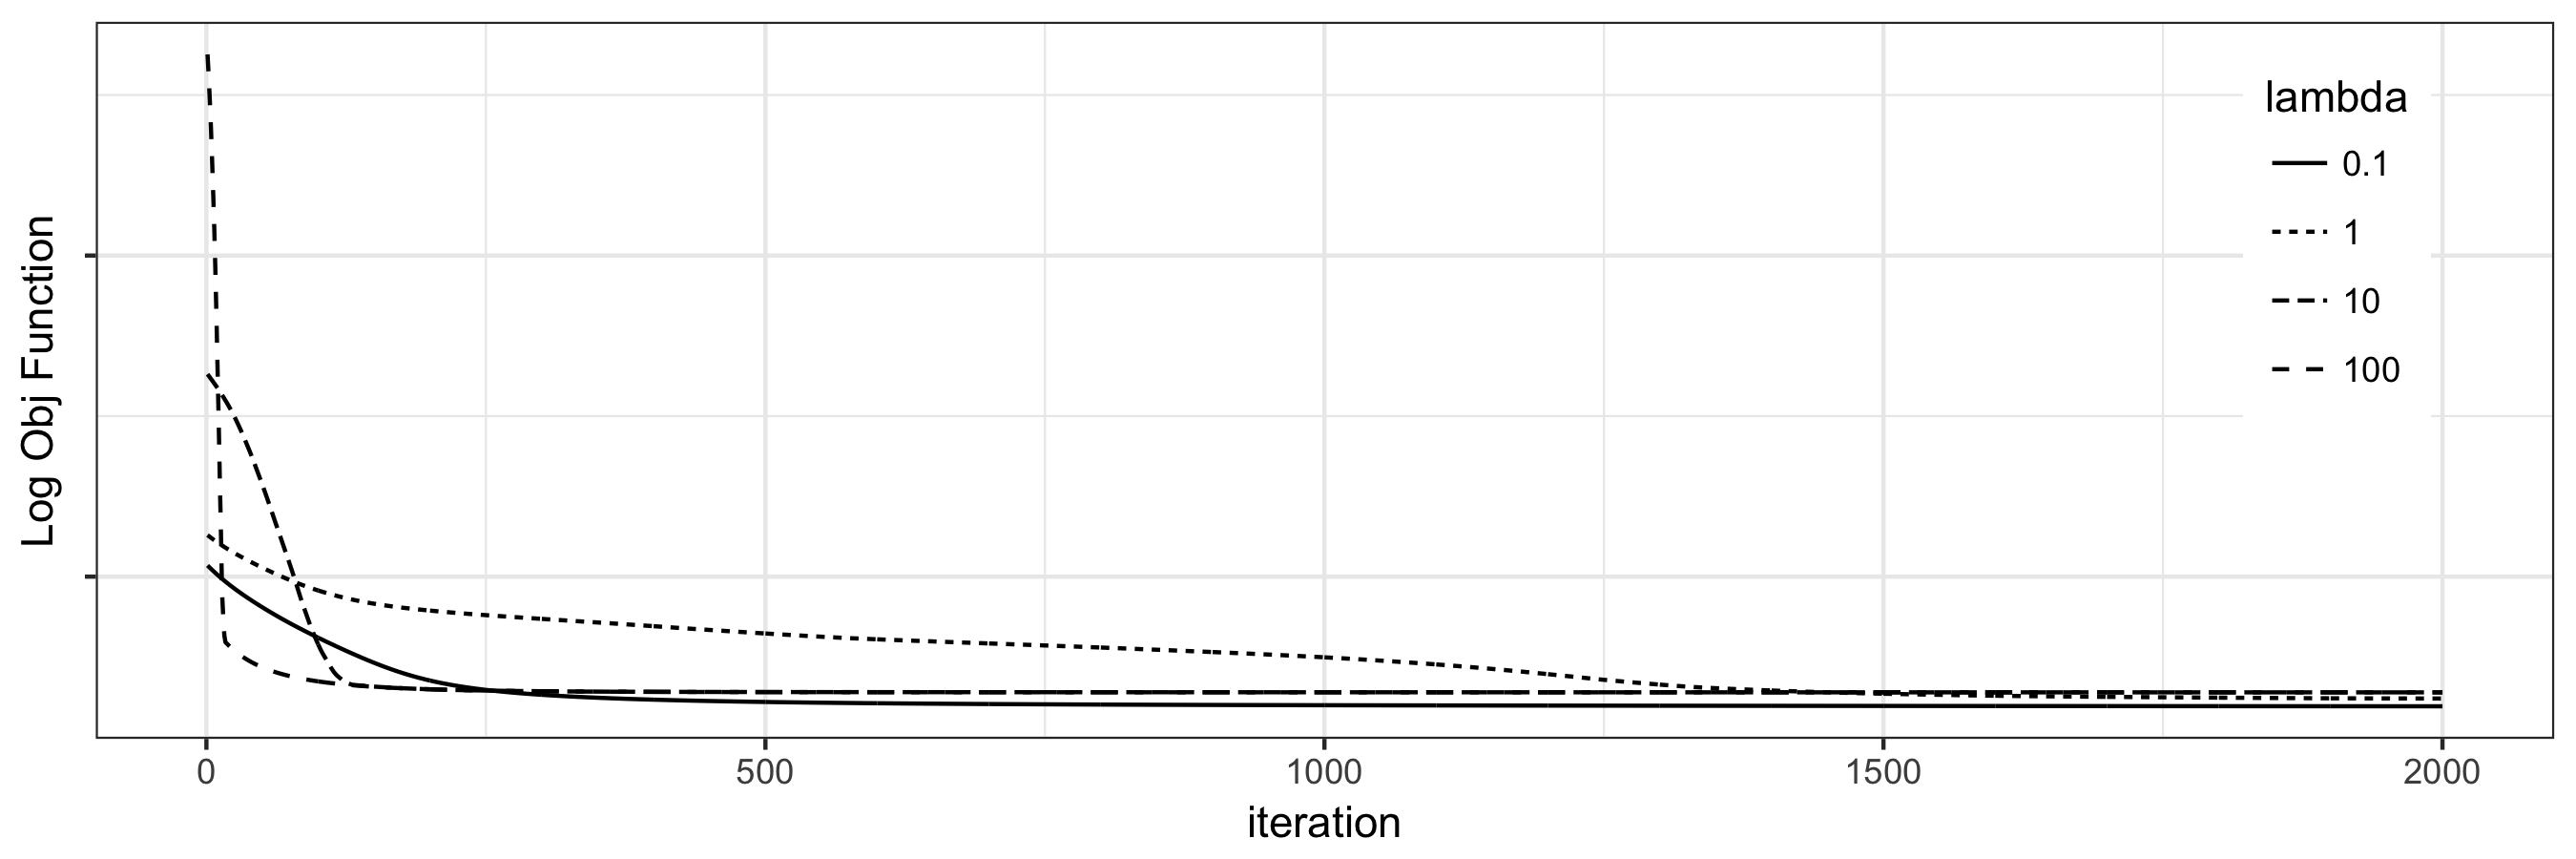
\includegraphics[width=20in]{../R/plot_objective.png} % requires the graphicx package
   \caption{Objective function for different values of $\lambda$}
   \label{fig:obj_fun}
\end{figure}

\begin{figure}[h!]
   \centering
   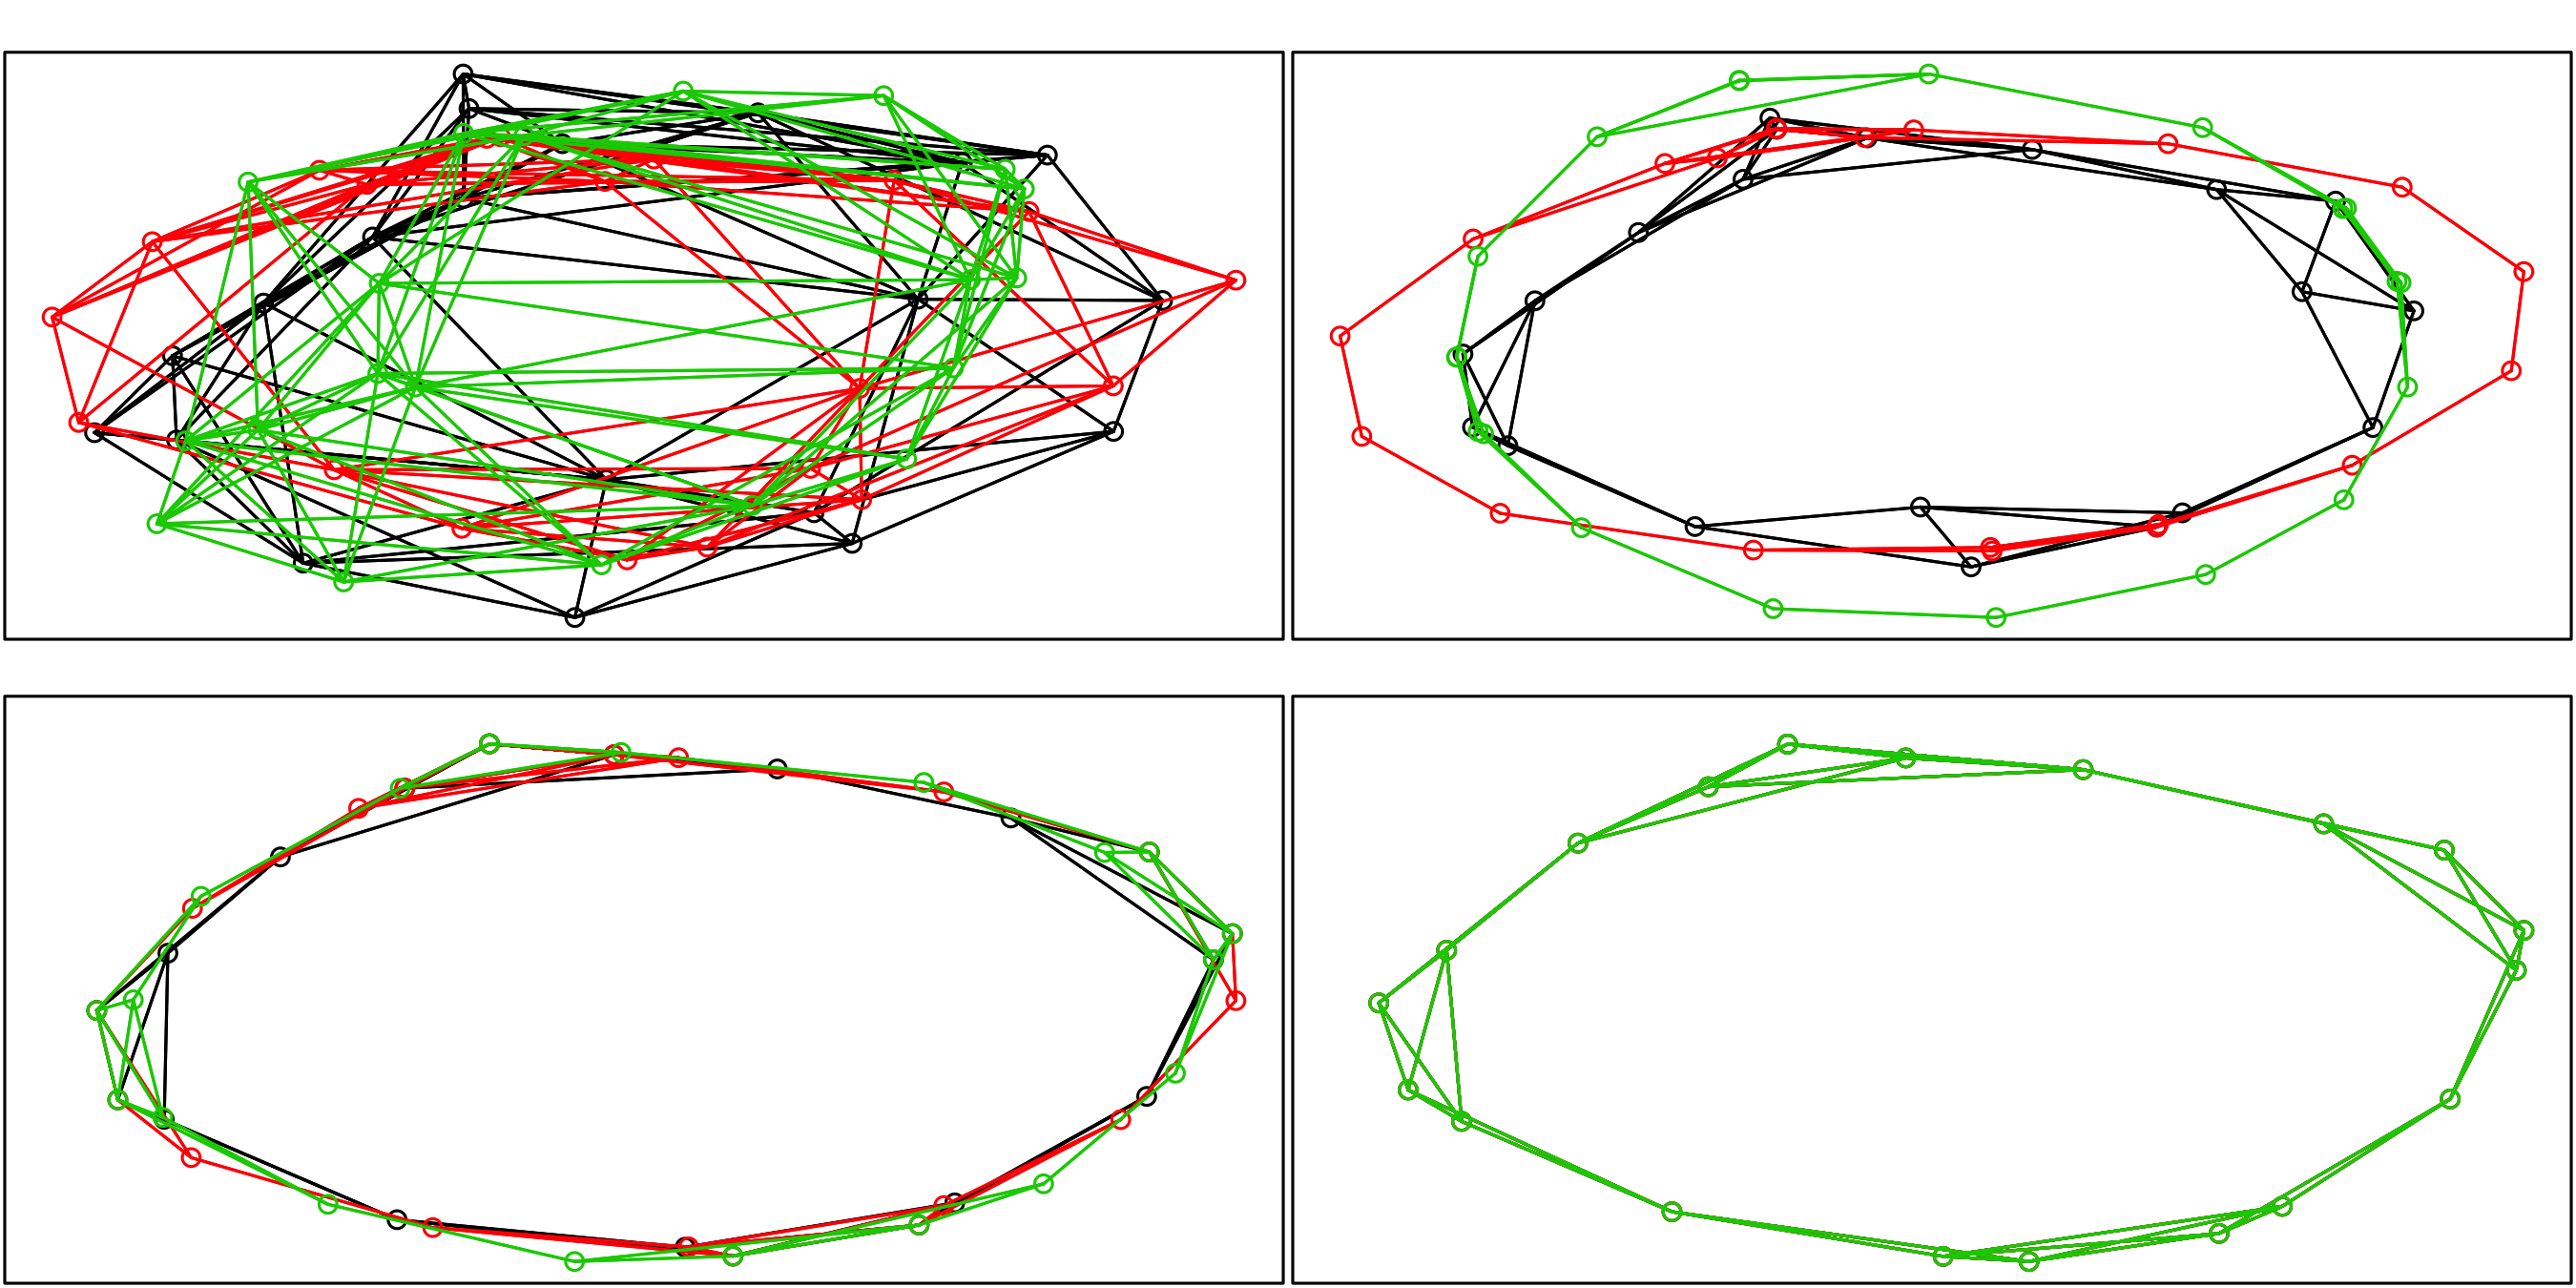
\includegraphics[width=19in]{../R/plot_positions.png} % requires the graphicx package
   \caption{Initial and final positions using $\lambda=1$}
   \label{fig:positions}
\end{figure}


%\begin{figure}
%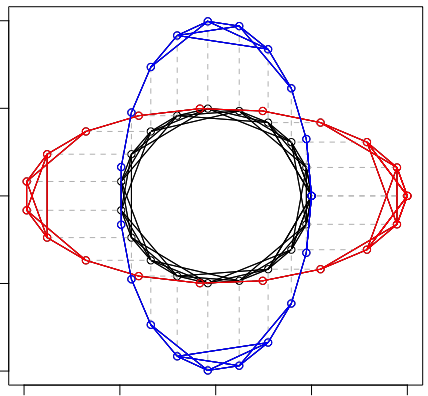
\includegraphics[width=0.8\linewidth]{error_daisy}
%\caption{Figure caption}
%\end{figure}

\end{block}

%----------------------------------------------------------------------------------------

\begin{columns}[t,totalwidth=\twocolwid] % Split up the two columns wide column again

\begin{column}{\onecolwid} % The first column within column 2 (column 2.1)

%----------------------------------------------------------------------------------------
%	MATHEMATICAL SECTION
%----------------------------------------------------------------------------------------

%\begin{block}{Model's Advantages}

%Our model has the additional inclusion of a hierarchy on the latent variables:
%\[
%z_{ik} = b_i + \epsilon_{ik}
%\]
%
%each node has a separate latent position to explain its ties within a
%single layer of the multigraph, but these multiple positions are all
%tied together by a single ``base'' position for that node $b_i$, and a
%layer-specific perturbation, $\epsilon_{ik}$.
%
%This allows two major advantages. One is graph-wise regularization
%with a group lasso penalty, allowing entire redundant layers to be
%removed for meaningful dimensionality reduction. Second,
%regularization allows a manual tuning between layouts that are
%expressive, and those that are comparable, solving the difficult
%problem of visual comparability.
%
%\end{block}

%----------------------------------------------------------------------------------------

\end{column} % End of column 2.1

\begin{column}{\onecolwid} % The second column within column 2 (column 2.2)

%----------------------------------------------------------------------------------------

\end{column} % End of column 2.2

\end{columns} % End of the split of column 2

\end{column} % End of the second column

\begin{column}{\sepwid}\end{column} % Empty spacer column

\begin{column}{\onecolwid} % The third column

  \begin{block}{Objective Functions}
    \begin{figure}[h!]
   \centering
   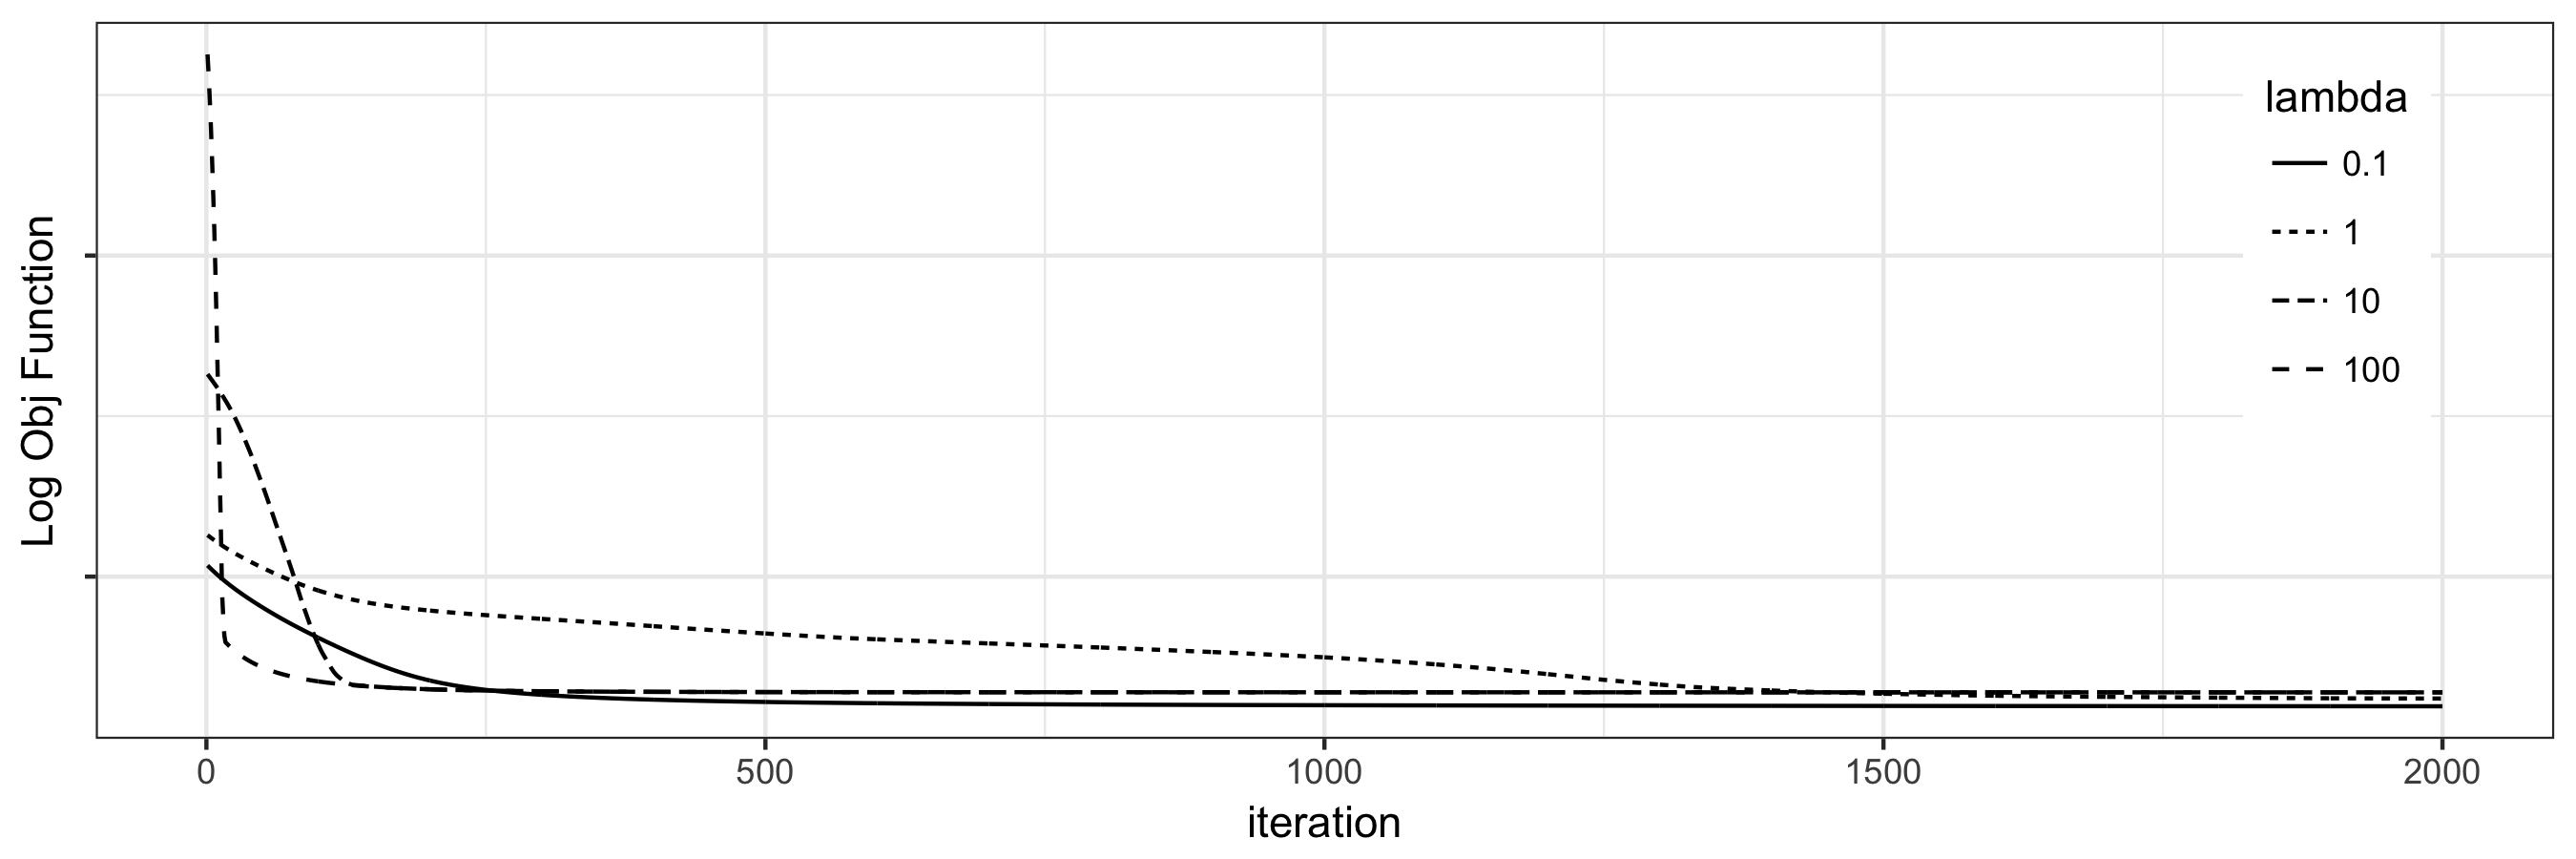
\includegraphics[width=\textwidth]{../R/plot_objective.png} % requires the graphicx package
   \caption{Objective function for different values of $\lambda$}
   \label{fig:obj_fun}
\end{figure}

  \end{block}

  \begin{block}{Challenges}

    \begin{itemize}
    \item Negative log-likelihood is not convex in the positions\\
      \textbf{Fix:} We started from carefully chosen initializations
    \item Distances between positions will yield same likelihood under
      translations and rotation\\
      \textbf{Fix:} Fit coordinate-wise, not allowing for spin, unlike the
      standard sampling approaches
    \end{itemize}
% \begin{figure}
% \centering
% 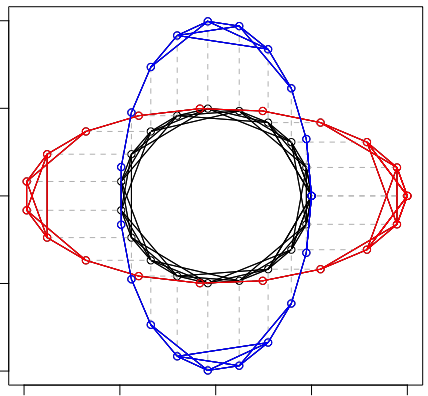
\includegraphics{error_daisy}
% \caption{A Stylized Multigraph}
% \end{figure}

\end{block}

%----------------------------------------------------------------------------------------
%	ADDITIONAL INFORMATION
%----------------------------------------------------------------------------------------

%\begin{block}{Paths}
%
% \textbf{Weeks gestation:}
%
%\end{block}


%----------------------------------------------------------------------------------------
%	CONCLUSION
%----------------------------------------------------------------------------------------

\begin{block}{Conclusion}

We found that proximal gradient methods are an effective tool for
refining an HLSM fit, given a good starting point.


\end{block}


%----------------------------------------------------------------------------------------
%	REFERENCES
%----------------------------------------------------------------------------------------

 \begin{block}{References}

 \nocite{*} % Insert publications even if they are not cited in the poster
 \small{\bibliographystyle{unsrt}
 \bibliography{sample}\vspace{0.75in}}

Hoff, Peter D., Adrian E. Raftery, and Mark S. Handcock. \textit{Latent space approaches to social network analysis.} Journal of the american Statistical association 97.460 (2002): 1090-1098.\\
%\\
Salter-Townshend, Michael, and Tyler H. McCormick. \textit{Latent space models for multiview network data}. Technical Report 622, Department of Statistics, University of Washington, 2013.\\
%\\
Salter-Townshend. M, \textit{Personal communication}, 2017\\
%\\
Bob Carpenter, Andrew Gelman, Matthew D. Hoffman, Daniel Lee, Ben Goodrich, Michael Betancourt, Marcus Brubaker, Jiqiang Guo, Peter Li, and Allen Riddell. \textit{Stan: A probabilistic programming language}. Journal of Statistical Software 76(1). DOI 10.18637/jss.v076.i01, 2017\\
%\\
Loewi, A., \textit{Parent-Teacher Relationships and Student Outcomes}, 2017


 \end{block}

%----------------------------------------------------------------------------------------
%	ACKNOWLEDGEMENTS
%----------------------------------------------------------------------------------------

%\setbeamercolor{block title}{fg=red,bg=white} % Change the block title color

\begin{block}{Acknowledgements}

  {\small\rmfamily{
      The authors would like to thank the Network Analysis group in the
      Department of Statistics and Data Science for their invitation to
      present, and the helpful feedback they contributed.
      }}

\end{block}

%----------------------------------------------------------------------------------------
%	CONTACT INFORMATION
%----------------------------------------------------------------------------------------

% \begin{columns}
%   \begin{column}{0.6\linewidth}
% %\setbeamercolor{block alerted title}{fg=black,bg=norange} % Change the alert block title colors
% %\setbeamercolor{block alerted body}{fg=black,bg=white} % Change the alert block body colors

% \begin{block}{Contact Information}

% \textbf{Corresponding author:} Octavio Mesner\\
% \textbf{Email:} \href{mailto:omesner@cmu.edu}{\texttt{omesner@cmu.edu}}\\
% \textbf{Address:} 129 Baker Hall, Pittsburgh, PA 15213

% \end{block}

%   \end{column}
%   \begin{column}{0.35\linewidth}
%     \includegraphics[width=.8\linewidth]{CMU_Logo_Stack_Red.eps}
%   \end{column}
% \end{columns}

%----------------------------------------------------------------------------------------

\end{column} % End of the third column

\end{columns} % End of all the columns in the poster

\end{frame}  % End of the enclosing frame

\end{document}
